\section{Realizzazione}

\subsection{Backend}

Il backend è diviso in due parti principali:
\begin{itemize}
	\item \textbf{Controller}: si occupa di gestire le richieste HTTP, che siano
		\texttt{POST} oppure \texttt{GET}. In particolare, si occupa di:
		\begin{enumerate}
			\item Controllare che l'utente abbia l'autorizzazione per effettuare la 
				richiesta;

			\item Controllare che i parametri della richiesta siano corretti;

			\item Sanitizzare i parametri della richiesta;

			\item Invocare i metodi corretti dal Model;

			\item Tornare la risposta al client, che sia un errore oppure un 
				risultato.
		\end{enumerate}

	\item \textbf{Model}: si occupa di gestire la logica dell'applicazione. In 
		particolare, si occupa di:
		\begin{enumerate}
			\item Interrogare il database;

			\item Definire e applicare le regole di business;

			\item Tornare i risultati al Controller.
		\end{enumerate}
\end{itemize}

\subsubsection{Controller}

Il Controller è composto da due classi principali:
\begin{itemize}
	\item \textbf{Router}: si occupa di individuare l'\texttt{Api} corretta, che
		si occupa di gestire la richiesta. In particolare, un \texttt{Router} è 
		composto da una lista di \texttt{Api}. In realtà, come si può vedere 
		in \texttt{index.php}, un \texttt{Router}, può essere composto anche da
		una lista di \texttt{Router}. Questo permette di creare un sistema di
		routing modulare, in cui ogni modulo ha il proprio \texttt{Router};
		\begin{figure}[H]
			\centering
			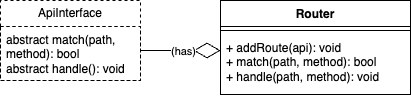
\includegraphics[width=0.5\textwidth]{figures/RouterClassDiagram.png}
			\caption{Struttura di un Router}
		\end{figure}

	\item \textbf{Api}: si occupa di gestire una specifica richiesta. In 
		particolare, una \texttt{Api} è composta da due metodi principali:
		\begin{itemize}
			\item \texttt{match()}: che ritorna \texttt{true} se l'\texttt{Api}
				è in grado di gestire la richiesta, \texttt{false} altrimenti;

			\item \texttt{handle()}: si occupa di invocare il metodo corretto 
				del Model e tornare il risultato al client.
		\end{itemize}

		Si noti che \texttt{Api} è una classe astratta, perché richiede
		l'implementazione del metodo \texttt{handle()}. Infatti, \texttt{Api}
		viene implementata da due classi: \texttt{JsonApi}, che si occupa di
		gestire le richieste \texttt{POST}; e \texttt{HtmlApi}, che si occupa di
		gestire le richieste \texttt{GET}.
		\begin{figure}[H]
			\centering
			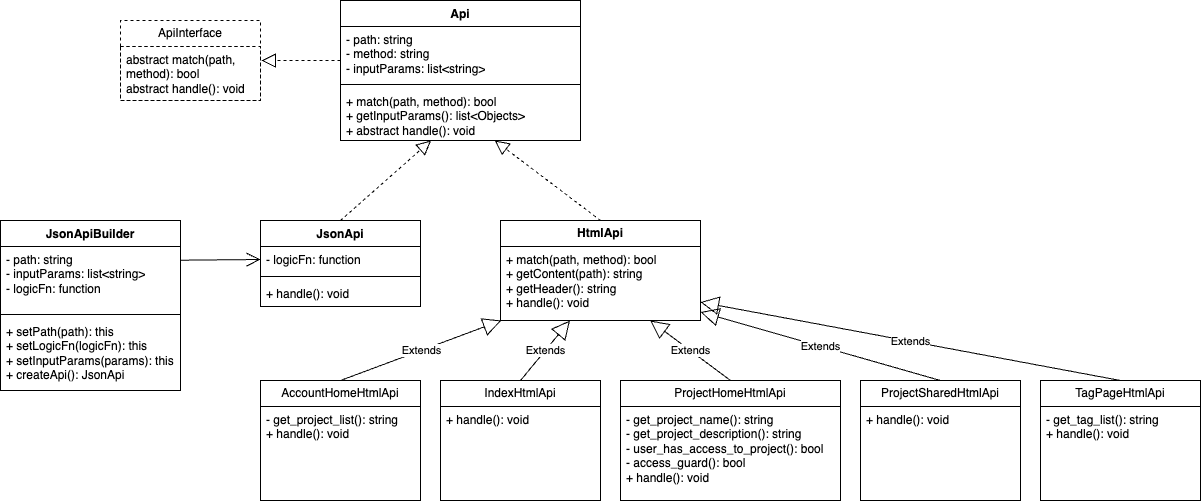
\includegraphics[width=0.9\textwidth]{figures/ApiClassDiagram.png}
			\caption{Gerarchia delle classi \texttt{Api}}
		\end{figure}
\end{itemize}

In particolare, \texttt{.htaccess} si occupa di reindirizzare tutte le richieste
a \texttt{index.php}, che utilizza un \texttt{Router} per gestire la richiesta.
In questo modo, gli URL messi a disposizione dall'applicazione risultano essere
più puliti e più facilmente gestibili, contribuendo alla \textit{Search Engine
Optimization}.

\subsubsection{Model}

Il Model è composto da due classi principali:
\begin{itemize}
	\item \textbf{Database}: si occupa di gestire la connessione al database e
		mettere a disposizione i metodi per interrogarlo. Di seguito, si 
		riportano i metodi principali:

		\begin{itemize}
			\item \texttt{getInstance()}: ritorna l'istanza del database,
				infatti \texttt{Database} è un \textit{Singleton};

			\item \texttt{query()}: esegue una query al database;

			\item \texttt{prepareAndBindParams()}: prepara una query al database
				e. La preparazione della query è necessaria per evitare 
				\textit{SQL injection};
	\end{itemize}

	\item \textbf{DatabaseManager}: le estensioni di questa classe si occupano
		di fornire la \textit{business logic} dell'applicazione. Sono omessi i
		parametri dei metodi, in quanto non sono rilevanti per la comprensione
		della struttura del Model. In particolare, le classi offrono i metodi di
		accesso al database.
\end{itemize}

\begin{figure}[H]
	\centering
	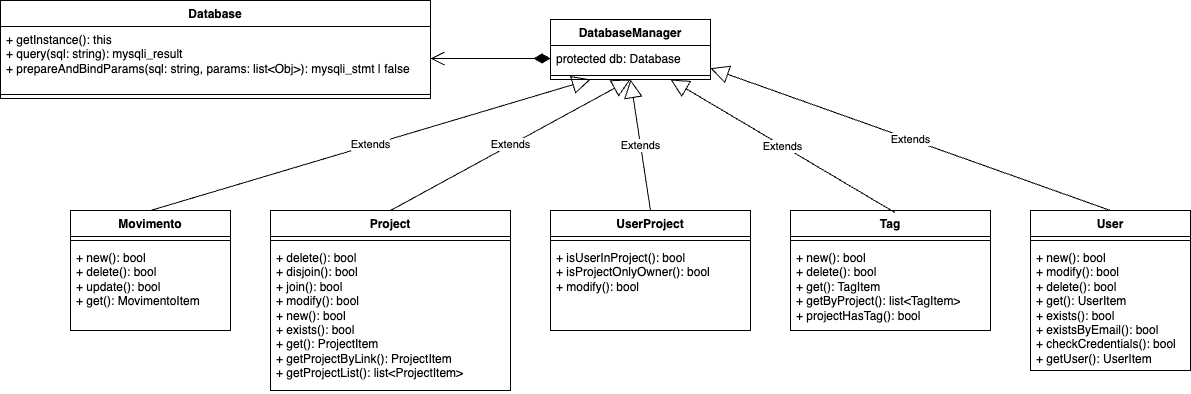
\includegraphics[width=0.9\textwidth]{figures/ModelClassDiagram.png}
	\caption{Struttura del \texttt{Model}}
\end{figure}

\subsubsection{Database}

\begin{figure}[H]
	\centering
	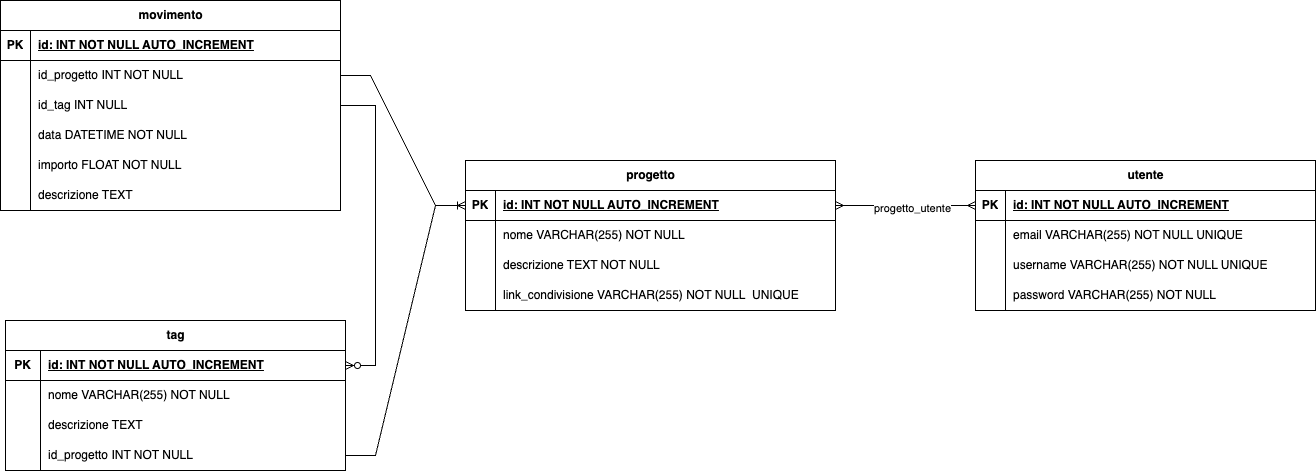
\includegraphics[width=0.9\textwidth]{figures/Database.png}
	\caption{Diagramma del database}
\end{figure}

Si noti che per quanto riguarda la gestione del database, sarebbe possibile
creare due \textit{instance} \texttt{tag} per il medesimo \texttt{progetto}. In 
realtà, la \textit{business logic} dell'applicazione non lo permette.
Per stabilire la connessione con il database viene utilizzata l'estensione
\texttt{MySQLi} di PHP.

\subsection{Frontend}

Il frontend è stato sviluppato utilizzando il pattern architetturale
\textit{Model View Controller}. Questa scelta è stata fatta per separare la
struttura, la presentazione e il comportamento dell'applicazione, che permette 
di migliorare il mantenimento del
codice, la scalabilità e la riusabilità. Non solo, ma migliora anche il
\textit{ranking} nei motori di ricerca, in quanto i motori di ricerca
considerano il peso delle pagine web, e una struttura ben organizzata permette
di ridurne le dimensioni.\\
In particolare, la scelta architetturale è evidenziata dalla gestione dei
\textit{feedback} e dell'interazione con i canvas, perché il resto
dell'applicazione è gestito dal backend.

\subsubsection{\textit{Responsiveness}}

Per ottenere un design \textit{responsive} sono stati definiti quattro 
\textit{breakpoint}:
\begin{itemize}
	\item \textbf{Mobile}: per schermi con larghezza inferiore a 483px;

	\item \textbf{Tablet in modalità verticale}: per schermi con larghezza 
		compresa tra 484px e 600px;

	\item \textbf{Tablet in modalità orizzontale o laptop piccoli}: per schermi 
		con larghezza compreso tra 601px e 1280px;

	\item \textbf{Desktop}: per schermi con larghezza superiore a 1281px.
\end{itemize}

\subsubsection{\textit{Feedback}}

Per gestire i \textit{feedback} viene definita una funzione che intercetta tutte
le chiamate \texttt{POST} al server, ovvero tutti gli \texttt{input} con 
\texttt{type="submit"}. In particolare, la funzione si occupa di:
\begin{enumerate}
	\item Invocare la funzione \texttt{postRequest()}, che si occupa di inviare
		la richiesta al server, estraendo i dati dall'\texttt{event} passato;

	\item Gestire la risposta del server, mostrando un messaggio di errore o di
		successo, ovvero viene aggiornata la \textit{View} dal 
		\textit{Controller}.
\end{enumerate}

\subsubsection{Canvas}

Per gestire i canvas è definita una classe \texttt{TransazioniSingleton}, che si
occupa dei seguenti compiti:
\begin{itemize}
	\item Mantenere la lista delle transazioni aggiornata;

	\item Ricordare il periodo di tempo selezionato;

	\item Ricordare i tag selezionati;

	\item Notificare le funzioni che si sono registrate per ricevere le 
		transazioni non appena queste sono aggiornate.
\end{itemize}

Dunque la classe \texttt{TransazioniSingleton} utilizza due \textit{desing
pattern}: \textit{Singleton} e \textit{Observer}. In particolare, il
\textit{Singleton} permette di avere una sola istanza della classe, mentre
l'\textit{Observer} permette di notificare le funzioni che si sono registrate
per ricevere le transazioni non appena queste sono aggiornate.\\
Le funzioni che si registrano per ricevere le transazioni sono le seguenti:
\begin{itemize}
	\item \texttt{drawChart()}: si occupa di disegnare il canvas all'interno
		della pagina "Project Home";

	\item \texttt{drawCakeChart()}: si occupa di disegnare il canvas all'interno
		della pagina "Project Cake";

	\item \texttt{updateTransazioniTable()}: si occupa di aggiornare la tabella
		con le transazioni all'interno delle pagine "Project Home" e "Project
		Cake".
\end{itemize}










